\documentclass[12pt]{article}

\usepackage{sbc-template}
\usepackage[utf8]{inputenc}
\usepackage[T1]{fontenc}
\usepackage{graphicx,url}
\usepackage{booktabs,tabularx,array}
\usepackage{float}
\usepackage{xcolor}
\usepackage{listings}
\usepackage{tikz}
\usetikzlibrary{arrows.meta,positioning,fit,backgrounds,calc,shapes.geometric}
\usepackage[hidelinks]{hyperref}

% Português: usa o babel quando o pacote "babel-portuges" estiver instalado
% (Overleaf e TeX Live completo). Sem ele, define os nomes manualmente.
\IfFileExists{portuges.ldf}{%
  \usepackage[brazil]{babel}%
}{%
  \renewcommand{\refname}{Referências}%
  \renewcommand{\figurename}{Figura}%
  \renewcommand{\tablename}{Tabela}%
  \hyphenpenalty=10000\exhyphenpenalty=10000%
}

\sloppy
\emergencystretch=2em
% O template usa \flushbottom; com figuras fixas ([H]) isso gera espaços enormes.
\raggedbottom

\lstset{
  basicstyle=\ttfamily\footnotesize,
  columns=fullflexible,
  keepspaces=true,
  breaklines=true,
  frame=single,
  rulecolor=\color{black!30},
  xleftmargin=0.5em,
  xrightmargin=0.5em,
  aboveskip=6pt,
  belowskip=6pt,
  literate={á}{{\'a}}1 {ã}{{\~a}}1 {â}{{\^a}}1 {é}{{\'e}}1 {ê}{{\^e}}1 {í}{{\'i}}1
           {ó}{{\'o}}1 {õ}{{\~o}}1 {ô}{{\^o}}1 {ú}{{\'u}}1 {ç}{{\c c}}1 {→}{{$\rightarrow$}}1
}

\newcommand{\cod}[1]{\texttt{#1}}

\title{Integração entre i-Educar e Moodle:\\ uma aplicação monolítica de sincronização}

\author{Nathalie Jordão\inst{1}, Yasmin Weber\inst{1}}

\address{Disciplina de Projeto e Arquitetura de Software -- Trabalho T1, Entrega 2}

\begin{document}

\maketitle

\begin{resumo}
Este relatório descreve a implementação da integração planejada na Entrega 1
entre o sistema de gestão escolar i-Educar e o ambiente virtual de
aprendizagem Moodle. A solução é uma aplicação monolítica em Python (FastAPI)
que lê turmas, alunos e matrículas pela API REST existente do i-Educar e os
cria e mantém no Moodle como cursos, usuários e inscrições, usando os serviços
web REST do Moodle, sem alterar nenhum dos dois sistemas. O ambiente completo
(i-Educar, Moodle, bancos de dados e a aplicação) é configurado com Docker
Compose. A sincronização é periódica e também pode ser disparada manualmente,
é idempotente (não duplica registros), envia ao Moodle apenas o que mudou e
isola falhas por registro. Os testes contra instâncias reais do i-Educar 2.12
e do Moodle 5.0.2 sincronizaram 2 escolas, 21 turmas, 210 alunos e 210
matrículas sem erros e validaram atualização, transferência, remanejamento,
e-mails duplicados, recriação de registros apagados e indisponibilidade dos
sistemas.
\end{resumo}

% ============================================================================
\section{Objetivo da integração}

Em uma rede de ensino que usa o i-Educar para a gestão acadêmica e o Moodle
como ambiente virtual, a mesma turma e os mesmos alunos precisariam ser
cadastrados duas vezes. O objetivo da integração, definido na Entrega 1, é
\textbf{evitar esse recadastro}: o i-Educar é a fonte oficial dos dados
escolares e o Moodle passa a refletir automaticamente as turmas, os alunos e
os vínculos de matrícula, inclusive quando eles mudam ao longo do ano
(correções de nome, transferências, remanejamentos).

A Tabela~\ref{tab:entrega1} relaciona as decisões do planejamento com o que foi
implementado.

\begin{table}[H]
\centering
\caption{Planejamento (Entrega 1) e implementação (Entrega 2)}
\label{tab:entrega1}
\footnotesize
\begin{tabularx}{\linewidth}{>{\raggedright\arraybackslash}p{3.3cm}>{\raggedright\arraybackslash}X>{\raggedright\arraybackslash}X}
\toprule
\textbf{Questão} & \textbf{Entrega 1} & \textbf{Entrega 2} \\
\midrule
O que integrar & Turmas em cursos, alunos em usuários, vínculos em inscrições & Implementado; escolas também viram categorias, para organizar os cursos \\
Fonte dos dados & \cod{pmieducar.turma}, \cod{aluno}, \cod{cadastro.pessoa}, \cod{matricula}, \cod{matricula\_turma} & Mesmas tabelas, lidas pela API REST do i-Educar \\
Quando & Periódico (5 min) e manual & Agendador interno (5 min), botão no painel e \cod{POST /sincronizacoes} \\
Como obter os dados & API existente, sem alterar o i-Educar & API autenticada por token (Laravel Sanctum) \\
No Moodle & Serviços web REST e conta autorizada & Configuração automática: REST, papel mínimo, usuário e token \\
Arquitetura & Programa separado (microsserviço) & Aplicação monolítica única, conforme o enunciado da Entrega 2 (Seção~\ref{sec:decisoes}) \\
Situação prática & Docker pendente & Ambiente completo em Docker Compose \\
\bottomrule
\end{tabularx}
\end{table}

% ============================================================================
\section{Informações sincronizadas}
\label{sec:dados}

A sincronização tem sentido único (i-Educar $\rightarrow$ Moodle) e considera
um ano letivo (o atual, por padrão). Cada registro criado no Moodle recebe no
campo \cod{idnumber} um identificador derivado da chave de origem, o que
permite reencontrá-lo depois. A Tabela~\ref{tab:mapeamento} resume o
mapeamento.

\begin{table}[H]
\centering
\caption{Mapeamento entre i-Educar e Moodle}
\label{tab:mapeamento}
\footnotesize
\begin{tabularx}{\linewidth}{>{\raggedright\arraybackslash}p{3.0cm}>{\raggedright\arraybackslash}p{1.8cm}>{\raggedright\arraybackslash}X}
\toprule
\textbf{i-Educar} & \textbf{Moodle} & \textbf{Regras de mapeamento} \\
\midrule
Escola (\cod{escola}) & Categoria de curso & \cod{idnumber = ieducar-escola-<cod>}; nome da escola \\
Turma (\cod{turma}) & Curso & \cod{idnumber = ieducar-turma-<cod>}; nome completo com turma, série e ano; nome breve único (\cod{<turma> <ano> \#<cod>}); categoria da escola; turma inativa vira curso oculto \\
Aluno (\cod{aluno} + \cod{pessoa}) & Usuário & \cod{idnumber = ieducar-aluno-<cod>}; \cod{username = aluno<cod>}; nome separado em nome e sobrenome; e-mail da pessoa ou e-mail técnico quando ausente, inválido ou já usado por outro aluno \\
Matrícula + enturmação (\cod{matricula},\newline \cod{matricula\_turma}) & Inscrição manual (estudante) & Curso da enturmação vigente; inscrição \textbf{ativa} se a matrícula está ativa e em andamento (cursando ou em exame); \textbf{suspensa} se transferida, abandonada, concluída ou excluída \\
\bottomrule
\end{tabularx}
\end{table}

Dados pessoais sensíveis, como CPF, data de nascimento e filiação, não são
lidos nem enviados ao Moodle: o nome de usuário é derivado do código do aluno,
e não do CPF, seguindo o princípio de minimização da LGPD~\cite{lgpd}.

% ============================================================================
\section{Arquitetura}
\label{sec:arquitetura}

\subsection{Visão geral}

A Figura~\ref{fig:arquitetura} mostra os containers do ambiente. A aplicação
de integração é um único processo (um monólito) que se comunica com o i-Educar
e com o Moodle apenas pelas APIs HTTP públicas de cada um. Os tokens de acesso
são gerados automaticamente pelos containers do i-Educar e do Moodle no
primeiro boot e entregues à integração por um volume compartilhado, somente
leitura para ela.

\begin{figure}[H]
\centering
\resizebox{\linewidth}{!}{%
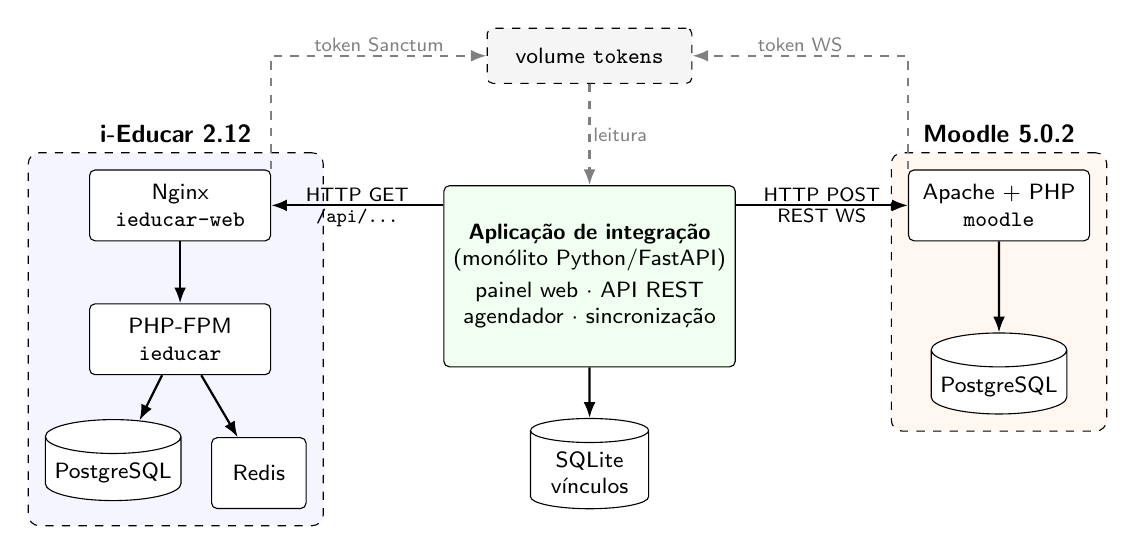
\begin{tikzpicture}[
  font=\sffamily\footnotesize,
  box/.style={draw, rounded corners=2pt, align=center, minimum height=0.9cm, fill=white},
  db/.style={draw, cylinder, shape border rotate=90, aspect=0.25, align=center, minimum height=0.9cm, minimum width=1.5cm, fill=white},
  grp/.style={draw, dashed, rounded corners=4pt, inner sep=6pt},
  arr/.style={-{Latex[length=2mm]}, thick},
  lbl/.style={font=\sffamily\scriptsize, align=center, inner sep=1pt}
]
  % i-Educar
  \node[box, minimum width=2.3cm] (iweb) at (0,0) {Nginx\\\cod{ieducar-web}};
  \node[box, minimum width=2.3cm] (iphp) at (0,-1.7) {PHP-FPM\\\cod{ieducar}};
  \node[db] (idb) at (-0.85,-3.4) {PostgreSQL};
  \node[box, minimum width=1.2cm] (ired) at (1.0,-3.4) {Redis};
  \begin{scope}[on background layer]
    \node[grp, fill=blue!4, fit=(iweb)(iphp)(idb)(ired), label={[font=\sffamily\bfseries\small]above:i-Educar 2.12}] {};
  \end{scope}

  % Integração
  \node[box, minimum width=3.7cm, minimum height=2.3cm, fill=green!6] (app) at (5.2,-0.9)
    {\textbf{Aplicação de integração}\\(monólito Python/FastAPI)\\[2pt]painel web $\cdot$ API REST\\agendador $\cdot$ sincronização};
  \node[db] (sqlite) at (5.2,-3.4) {SQLite\\vínculos};
  \node[box, dashed, minimum width=2.6cm, minimum height=0.7cm, fill=gray!8] (tok) at (5.2,1.9) {volume \cod{tokens}};

  % Moodle
  \node[box, minimum width=2.3cm] (moodle) at (10.4,0) {Apache + PHP\\\cod{moodle}};
  \node[db] (mdb) at (10.4,-2.3) {PostgreSQL};
  \begin{scope}[on background layer]
    \node[grp, fill=orange!6, fit=(moodle)(mdb), label={[font=\sffamily\bfseries\small]above:Moodle 5.0.2}] {};
  \end{scope}

  \draw[arr] (iweb) -- (iphp);
  \draw[arr] (iphp) -- (idb);
  \draw[arr] (iphp) -- (ired);
  \draw[arr] (moodle) -- (mdb);
  \draw[arr] (app) -- (sqlite);
  \draw[arr] (app.west |- iweb.east) -- node[lbl, above] {HTTP GET} node[lbl, below] {\cod{/api/...}} (iweb.east);
  \draw[arr] (app.east |- moodle.west) -- node[lbl, above] {HTTP POST} node[lbl, below] {REST WS} (moodle.west);
  \draw[arr, dashed, gray] (iweb.north east) |- node[lbl, pos=0.75, above] {token Sanctum} (tok.west);
  \draw[arr, dashed, gray] (moodle.north west) |- node[lbl, pos=0.75, above] {token WS} (tok.east);
  \draw[arr, dashed, gray] (tok) -- node[lbl, right] {leitura} (app);
\end{tikzpicture}%
}
\caption{Containers do ambiente (Docker Compose) e comunicação entre eles}
\label{fig:arquitetura}
\end{figure}

\subsection{Organização interna do monólito}

Internamente, a aplicação é um \emph{monólito modular} organizado em camadas,
com dependências sempre apontando para dentro (Figura~\ref{fig:camadas}).
A regra de negócio não conhece HTTP, banco de dados nem o formato das APIs:
ela trabalha sobre o \emph{modelo canônico} (\cod{Escola}, \cod{Turma},
\cod{Aluno}, \cod{Matricula}) e conversa com os sistemas externos por meio de
interfaces.

\begin{figure}[H]
\centering
\resizebox{\linewidth}{!}{%
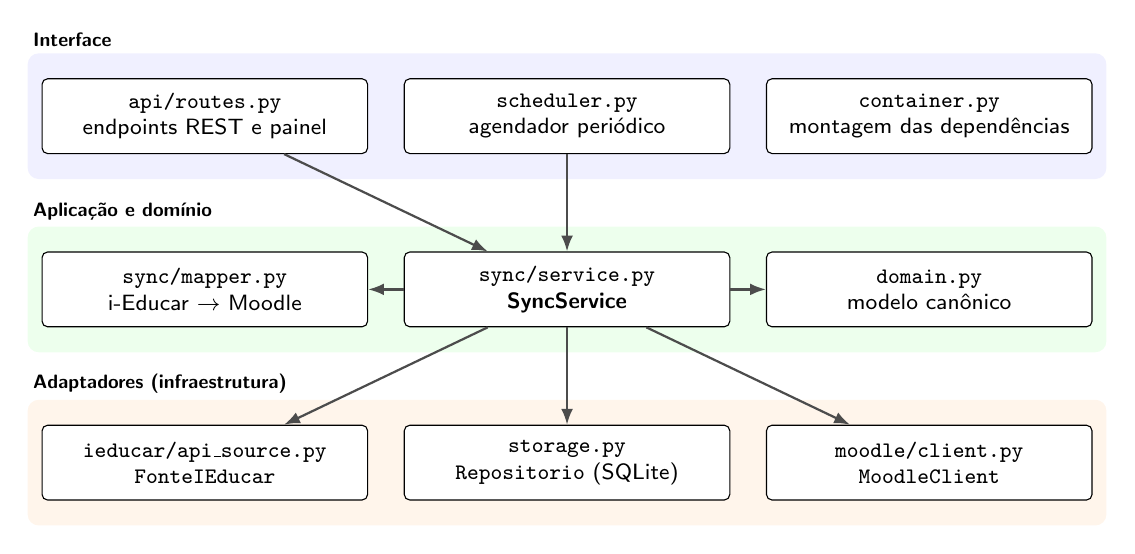
\begin{tikzpicture}[
  font=\sffamily\footnotesize,
  mod/.style={draw, rounded corners=2pt, align=center, minimum height=0.95cm, fill=white, text width=3.9cm},
  layer/.style={draw=none, rounded corners=4pt, inner sep=5pt},
  tag/.style={font=\sffamily\scriptsize\bfseries, anchor=south west, inner sep=2pt},
  arr/.style={-{Latex[length=2mm]}, thick, black!70}
]
  \node[mod] (rotas) at (0,0)  {\cod{api/routes.py}\\endpoints REST e painel};
  \node[mod] (agend) at (4.6,0)  {\cod{scheduler.py}\\agendador periódico};
  \node[mod] (cont)  at (9.2,0)  {\cod{container.py}\\montagem das dependências};

  \node[mod] (map)  at (0,-2.2) {\cod{sync/mapper.py}\\i-Educar $\rightarrow$ Moodle};
  \node[mod] (serv) at (4.6,-2.2) {\cod{sync/service.py}\\\textbf{SyncService}};
  \node[mod] (dom)  at (9.2,-2.2) {\cod{domain.py}\\modelo canônico};

  \node[mod] (fonte) at (0,-4.4) {\cod{ieducar/api\_source.py}\\\cod{FonteIEducar}};
  \node[mod] (repo)  at (4.6,-4.4) {\cod{storage.py}\\\cod{Repositorio} (SQLite)};
  \node[mod] (mcli)  at (9.2,-4.4) {\cod{moodle/client.py}\\\cod{MoodleClient}};

  \begin{scope}[on background layer]
    \node[layer, fill=blue!6, fit=(rotas)(cont), inner ysep=9pt] (l1) {};
    \node[layer, fill=green!7, fit=(map)(dom), inner ysep=9pt] (l2) {};
    \node[layer, fill=orange!8, fit=(fonte)(mcli), inner ysep=9pt] (l3) {};
  \end{scope}
  \node[tag] at (l1.north west) {Interface};
  \node[tag] at (l2.north west) {Aplicação e domínio};
  \node[tag] at (l3.north west) {Adaptadores (infraestrutura)};

  \draw[arr] (rotas) -- (serv);
  \draw[arr] (agend) -- (serv);
  \draw[arr] (serv) -- (map);
  \draw[arr] (serv) -- (dom);
  \draw[arr] (serv) -- (fonte);
  \draw[arr] (serv) -- (repo);
  \draw[arr] (serv) -- (mcli);
\end{tikzpicture}%
}
\caption{Camadas e módulos da aplicação de integração}
\label{fig:camadas}
\end{figure}

\subsection{Interfaces}

\textbf{Interface com o i-Educar (leitura).} O serviço depende apenas do
contrato \cod{FonteIEducar}, com dois métodos: \cod{verificar()} e
\cod{carregar(ano)}, que devolve escolas, turmas, alunos e matrículas já no
modelo canônico. A implementação usa a API do i-Educar~\cite{ieducar}
autenticada por \emph{bearer token} do Laravel Sanctum~\cite{sanctum}:

\begin{lstlisting}
GET /api/school?include=person:nome                    # escolas
GET /api/school-class?year_eq=2026&include=grade|course  # turmas
GET /api/registration?year_eq=2026&include=enrollments
    &only=pmieducar.matricula.ativo,...,nome,email   # matrículas
GET /api/version                                 # disponibilidade
\end{lstlisting}

\textbf{Interface com o Moodle (escrita).} O \cod{MoodleClient} encapsula o
protocolo REST do Moodle~\cite{moodlews} e usa somente funções nativas da
API~\cite{moodlewsapi}: \cod{core\_course\_get\_categories},
\cod{core\_course\_create\_categories}, \cod{core\_course\_update\_categories},
\cod{core\_course\_get\_courses\_by\_field}, \cod{core\_course\_create\_courses},
\cod{core\_course\_update\_courses}, \cod{core\_user\_get\_users\_by\_field},
\cod{core\_user\_create\_users}, \cod{core\_user\_update\_users},
\cod{enrol\_manual\_enrol\_users}, \cod{core\_enrol\_get\_enrolled\_users} e
\cod{core\_webservice\_get\_site\_info}.

\textbf{Interface da própria aplicação.} A Tabela~\ref{tab:endpoints} lista os
endpoints. A documentação OpenAPI é gerada automaticamente em \cod{/docs}.

\begin{table}[H]
\centering
\caption{Endpoints da aplicação de integração}
\label{tab:endpoints}
\footnotesize
\begin{tabularx}{\linewidth}{>{\raggedright\arraybackslash}p{6.3cm}>{\raggedright\arraybackslash}X}
\toprule
\textbf{Endpoint} & \textbf{Função} \\
\midrule
\cod{GET /} & Painel web: ações, totais vinculados e histórico \\
\cod{GET /health} & Verificação de vida (usada pelo Docker) \\
\cod{GET /saude} & Testa a comunicação com o i-Educar e o Moodle \\
\cod{POST /sincronizacoes} & Executa a sincronização e devolve o relatório (\cod{?completa=true}: reconciliação) \\
\cod{GET /sincronizacoes}, \cod{/sincronizacoes/\{id\}} & Histórico e detalhes, com erros por registro \\
\cod{GET /vinculos?tipo=} & Correspondências i-Educar $\leftrightarrow$ Moodle \\
\cod{GET /ieducar/dados} & Dados de origem já no modelo canônico \\
\cod{GET /moodle/turmas/\{id\}} & Curso e participantes de uma turma no Moodle \\
\bottomrule
\end{tabularx}
\end{table}

\subsection{Fluxo da sincronização}

A Figura~\ref{fig:fluxo} detalha uma execução, disparada pelo agendador (a
cada 5 minutos) ou manualmente. As entidades são processadas em ordem de
dependência: escolas, turmas, alunos e matrículas.

\begin{figure}[H]
\centering
\resizebox{\linewidth}{!}{%
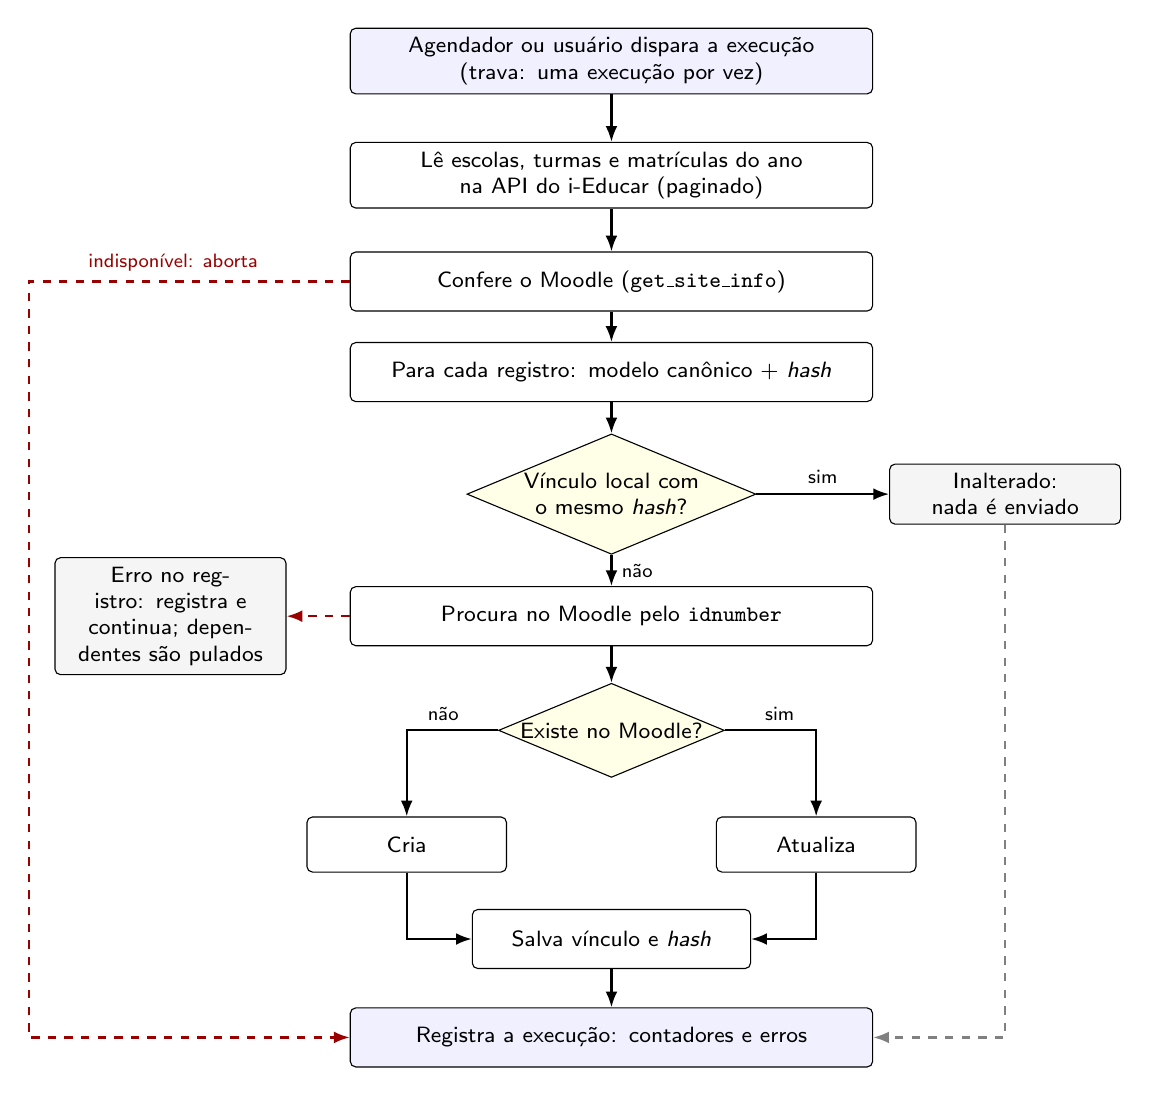
\begin{tikzpicture}[
  font=\sffamily\footnotesize,
  etapa/.style={draw, rounded corners=2pt, align=center, text width=6.4cm, minimum height=0.75cm, fill=white},
  curta/.style={draw, rounded corners=2pt, align=center, text width=2.3cm, minimum height=0.7cm, fill=white},
  dec/.style={draw, diamond, aspect=2.4, align=center, inner sep=0pt, fill=yellow!10, text width=2.4cm},
  ext/.style={draw, rounded corners=2pt, align=center, text width=2.7cm, minimum height=0.75cm, fill=gray!8},
  arr/.style={-{Latex[length=2mm]}, thick},
  lbl/.style={font=\sffamily\scriptsize}
]
  \node[etapa, fill=blue!6] (ini) at (0,0) {Agendador ou usuário dispara a execução\\(trava: uma execução por vez)};
  \node[etapa] (ler) at (0,-1.45) {Lê escolas, turmas e matrículas do ano\\na API do i-Educar (paginado)};
  \node[etapa] (sit) at (0,-2.8) {Confere o Moodle (\cod{get\_site\_info})};
  \node[etapa] (map) at (0,-3.95) {Para cada registro: modelo canônico + \emph{hash}};
  \node[dec] (hash) at (0,-5.5) {Vínculo local com o mesmo \emph{hash}?};
  \node[etapa] (busca) at (0,-7.05) {Procura no Moodle pelo \cod{idnumber}};
  \node[dec] (existe) at (0,-8.5) {Existe no Moodle?};
  \node[curta] (cria) at (-2.6,-9.95) {Cria};
  \node[curta] (atu) at (2.6,-9.95) {Atualiza};
  \node[etapa, text width=3.3cm] (salva) at (0,-11.15) {Salva vínculo e \emph{hash}};
  \node[etapa, fill=blue!6] (fim) at (0,-12.4) {Registra a execução: contadores e erros};

  \node[ext] (pula) at (5.0,-5.5) {Inalterado:\\nada é enviado};
  \node[ext] (err) at (-5.6,-7.05) {Erro no registro: registra e continua; dependentes são pulados};

  \draw[arr] (ini) -- (ler);
  \draw[arr] (ler) -- (sit);
  \draw[arr] (sit) -- (map);
  \draw[arr] (map) -- (hash);
  \draw[arr] (hash) -- node[lbl, right] {não} (busca);
  \draw[arr] (hash) -- node[lbl, above] {sim} (pula);
  \draw[arr] (busca) -- (existe);
  \draw[arr] (existe.west) -| node[lbl, above, pos=0.3] {não} (cria.north);
  \draw[arr] (existe.east) -| node[lbl, above, pos=0.3] {sim} (atu.north);
  \draw[arr] (cria.south) |- (salva.west);
  \draw[arr] (atu.south) |- (salva.east);
  \draw[arr] (salva) -- (fim);
  \draw[arr, dashed, red!60!black] (busca.west) -- (err.east);
  \draw[arr, dashed, gray] (pula.south) |- (fim.east);
  \draw[arr, dashed, red!60!black] (sit.west) -- node[lbl, above, pos=0.55] {indisponível: aborta} (-7.4,-2.8) |- (fim.west);
\end{tikzpicture}%
}
\caption{Fluxo de uma execução da sincronização}
\label{fig:fluxo}
\end{figure}

Para matrículas, a operação é a inscrição manual no curso da turma, ativa ou
suspensa conforme a situação. Se a enturmação mudou de turma (remanejamento),
a inscrição no curso antigo é suspensa antes da nova. Matrículas que já foram
sincronizadas e deixaram de existir na origem também são suspensas.

% ============================================================================
\section{Decisões técnicas}
\label{sec:decisoes}

\textbf{Aplicação monolítica.} A Entrega 1 previa um ``pequeno programa
separado''; o enunciado da Entrega 2 pede uma aplicação monolítica. A solução
mantém a integração fora do i-Educar e do Moodle (baixo acoplamento), mas
reúne comunicação, regras, agendamento, persistência e interface em um único
projeto, processo e implantação. Para o tamanho do problema isso simplifica a
operação (um container, um log, uma versão) e mantém as regras de consistência
em uma só transação lógica~\cite{richards2020}. A divisão em módulos com
interfaces explícitas permitiria extrair partes no futuro, se necessário.

\textbf{Python e FastAPI.} Código conciso para a lógica de integração,
cliente HTTP maduro (\cod{httpx}) e documentação OpenAPI gerada
automaticamente~\cite{fastapi}, útil na demonstração.

\textbf{Leitura pela API do i-Educar, sem alterá-lo.} Atende ao planejamento
e respeita as permissões do sistema. Foi necessário um ajuste: o endpoint de
matrículas faz \emph{JOIN} com \cod{aluno} e \cod{pessoa} para ordenar por
nome, o que torna a coluna \cod{ativo} ambígua. A integração pede as colunas
com o nome qualificado (\cod{only=pmieducar.matricula.ativo,\ldots}), o que
também traz nome e e-mail do aluno na mesma consulta. A escolha foi validada
contra a instância real.

\textbf{Sincronização por consulta periódica.} O i-Educar não oferece
eventos ou \emph{webhooks}; a consulta periódica (padrão \emph{polling
consumer}~\cite{hohpe2003}) a cada 5 minutos atende ao planejamento sem
modificar a origem.

\textbf{Prevenção de duplicidades em três níveis.} (1) O \cod{idnumber} no
Moodle é a chave natural da integração; antes de criar, o registro é procurado
por ele. (2) Uma tabela local de vínculos guarda a correspondência e o
\emph{hash} do último envio, evitando chamadas desnecessárias. (3) Uma trava
impede execuções concorrentes (a API responde HTTP 409). Se a base local for
perdida, os registros são reencontrados pelo \cod{idnumber} e apenas
revinculados.

\textbf{Reconciliação completa.} O atalho por \emph{hash} não percebe
alterações feitas diretamente no Moodle. Por isso existe a execução
\emph{completa}, que ignora o cache e confere todos os registros, recriando o
que tiver sido apagado; ela roda a cada 12 execuções agendadas (1 hora) e pode
ser disparada manualmente.

\textbf{Suspender em vez de remover.} Transferências, abandonos e
remanejamentos suspendem a inscrição. O aluno perde o acesso, mas o histórico
de atividades e notas no Moodle é preservado.

\textbf{Privilégio mínimo no Moodle.} A configuração automática cria um papel
\cod{integracao\_ieducar} apenas com as capacidades necessárias, um usuário de
serviço e um serviço externo restrito às 13 funções usadas. O token é
permanente e só desse serviço; não se usa a conta de administrador.

\textbf{SQLite para o estado da integração.} O estado é pequeno (vínculos e
histórico) e acessado por um único processo; o arquivo fica em um volume
Docker, sem exigir mais um servidor de banco.

\textbf{Tratamento de falhas.} Falhas de rede e respostas 5xx ou 429 são
repetidas com espera exponencial. Erros de um registro são isolados e
registrados; registros dependentes (por exemplo, matrículas de uma turma que
falhou) são pulados com o motivo e refeitos na execução seguinte, porque não
gravam vínculo. Se o Moodle ou o i-Educar estiverem fora do ar, a execução é
interrompida imediatamente e registrada como falha, sem tentar cada registro.

\textbf{E-mails.} O Moodle não aceita duas contas com o mesmo e-mail, e no
i-Educar é comum irmãos usarem o e-mail do responsável. Nesses casos, e
quando o e-mail falta ou é inválido, o aluno recebe um e-mail técnico
(\cod{aluno<cod>@sem-email.invalid}) e a sincronização não falha.

\textbf{Ambiente reprodutível.} O i-Educar é construído a partir do
repositório oficial em um \emph{commit} fixo, com as mesmas extensões do seu
Dockerfile, e é inicializado automaticamente (migrations, dados padrão,
dados de demonstração oficiais e token). O Moodle usa a imagem
\cod{bitnamilegacy/moodle:5.0.2}~\cite{bitnamimoodle} com um script que,
após a instalação, configura os serviços web. Tudo sobe com um único
\cod{docker compose up}~\cite{compose}.

A Tabela~\ref{tab:desafios} mostra como cada desafio antecipado na Entrega 1
foi tratado.

\begin{table}[H]
\centering
\caption{Desafios previstos na Entrega 1 e como foram tratados}
\label{tab:desafios}
\footnotesize
\begin{tabularx}{\linewidth}{>{\raggedright\arraybackslash}p{2.6cm}>{\raggedright\arraybackslash}X}
\toprule
\textbf{Desafio} & \textbf{Tratamento} \\
\midrule
Baixo acoplamento & Só APIs públicas; nenhum sistema foi alterado; regras isoladas do formato das APIs pelo modelo canônico \\
Compatibilidade & Mapeador dedicado: limites de tamanho, nomes em caixa alta normalizados, nome breve único, sobrenome obrigatório, e-mail técnico \\
Consistência & \cod{idnumber}, tabela de vínculos, \emph{hash}, trava de execução, suspensão de órfãos e reconciliação completa \\
Disponibilidade & Repetição com espera exponencial, interrupção rápida quando um sistema cai, refazer automático na execução seguinte \\
Segurança & Tokens gerados automaticamente e lidos de volume somente leitura; papel de privilégio mínimo; sem CPF e outros dados sensíveis \\
\bottomrule
\end{tabularx}
\end{table}

% ============================================================================
\section{Testes realizados}

\textbf{Testes automatizados.} São 54 testes (\cod{pytest}), executados com
\cod{docker compose exec integracao pytest}:
\begin{itemize}
  \item \emph{regras de sincronização} (21 testes), com um Moodle em memória que
    reproduz as restrições reais (unicidade de \cod{idnumber}, nome breve e
    e-mail; erro ao atualizar registro inexistente): criação, idempotência,
    perda da base local, reconciliação, atualização, e-mail repetido,
    transferência, remanejamento, órfãos, isolamento de falhas, refazer na
    execução seguinte, sistemas indisponíveis e concorrência;
  \item \emph{clientes HTTP} (15 testes), com respostas simuladas; as respostas do
    i-Educar são \emph{fixtures} capturadas da API real; cobrem formato dos
    parâmetros do Moodle, erros e avisos, repetição em 5xx/429, paginação,
    token recusado e escolha da enturmação vigente;
  \item \emph{mapeamento} (10 testes) e \emph{endpoints} (8 testes).
\end{itemize}

\textbf{Testes de integração com os sistemas reais.} Foram executados contra o
i-Educar 2.12.0 (mesmo \emph{commit} do Dockerfile, com o \emph{seeder} de
demonstração oficial: 2 escolas, 21 turmas e 210 alunos matriculados) e o
Moodle 5.0.2 (mesma versão da imagem), conferindo o resultado tanto pela
interface quanto diretamente no banco do Moodle. O roteiro foi:
\begin{enumerate}
  \item carga inicial e nova execução sem mudanças;
  \item alterações feitas no i-Educar como faria a secretaria: dois alunos novos
    matriculados, correção de um nome, uma transferência, um remanejamento de
    turma e dois irmãos com o mesmo e-mail;
  \item exclusão manual de um curso no Moodle, seguida de execução normal e de
    execução completa;
  \item Moodle fora do ar, i-Educar fora do ar e retorno ao normal;
  \item token inválido, execuções concorrentes e perda da base local da
    integração.
\end{enumerate}

% ============================================================================
\section{Resultados}

A Tabela~\ref{tab:resultados} resume as execuções do roteiro, registradas pela
própria aplicação.

\begin{table}[H]
\centering
\caption{Execuções contra o i-Educar e o Moodle reais}
\label{tab:resultados}
\footnotesize
\begin{tabularx}{\linewidth}{>{\raggedright\arraybackslash}p{3.1cm}>{\raggedright\arraybackslash}Xrr}
\toprule
\textbf{Cenário} & \textbf{Resultado} & \textbf{Status} & \textbf{Tempo} \\
\midrule
1. Carga inicial & 2 categorias, 21 cursos, 210 usuários e 210 inscrições criados & sucesso & 26,9 s \\
2. Sem mudanças & 443 registros inalterados; nenhuma escrita no Moodle & sucesso & 0,26 s \\
3. Alterações na origem & 2 alunos e 2 inscrições criados; 2 usuários atualizados (nome e e-mail); 1 inscrição movida (remanejamento); 1 suspensa (transferência) & sucesso & 0,67 s \\
4. Curso apagado no Moodle (normal) & Não detectado: registros inalterados & sucesso & 0,23 s \\
5. Mesmo caso (completa) & Curso recriado com as 10 inscrições; demais conferidos & sucesso & 18,2 s \\
6. Moodle fora do ar & Execução interrompida e registrada, sem tentar cada registro & falha & 1,7 s \\
7. i-Educar fora do ar & Execução interrompida e registrada & falha & 1,5 s \\
8. Sistemas de volta & Retomada normal, sem intervenção & sucesso & 0,3 s \\
\bottomrule
\end{tabularx}
\end{table}

Nos testes complementares, um token inválido do i-Educar foi identificado
como ``recusado (HTTP 401)''; uma segunda execução disparada durante outra
recebeu HTTP 409; e, após apagar a base local da integração, a execução
seguinte \emph{revinculou} os 443 registros pelo \cod{idnumber} sem criar
nenhuma duplicata no Moodle (as contagens de categorias, cursos e usuários
permaneceram 2, 21 e 210).

As Figuras~\ref{fig:ieducar} a~\ref{fig:painel} mostram a origem no i-Educar e
o resultado no Moodle ao final do roteiro.

\begin{figure}[H]
\centering
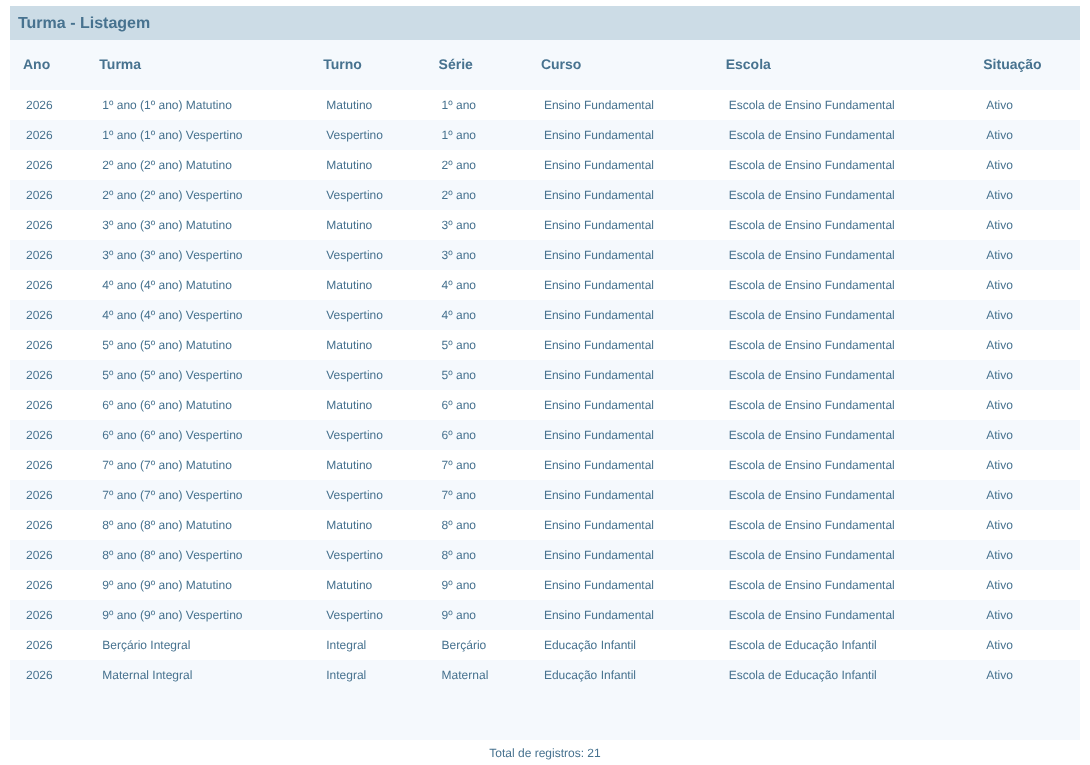
\includegraphics[width=0.92\linewidth]{figuras/ieducar_turmas.png}
\caption{Origem: turmas do ano letivo no i-Educar}
\label{fig:ieducar}
\end{figure}

\begin{figure}[H]
\centering
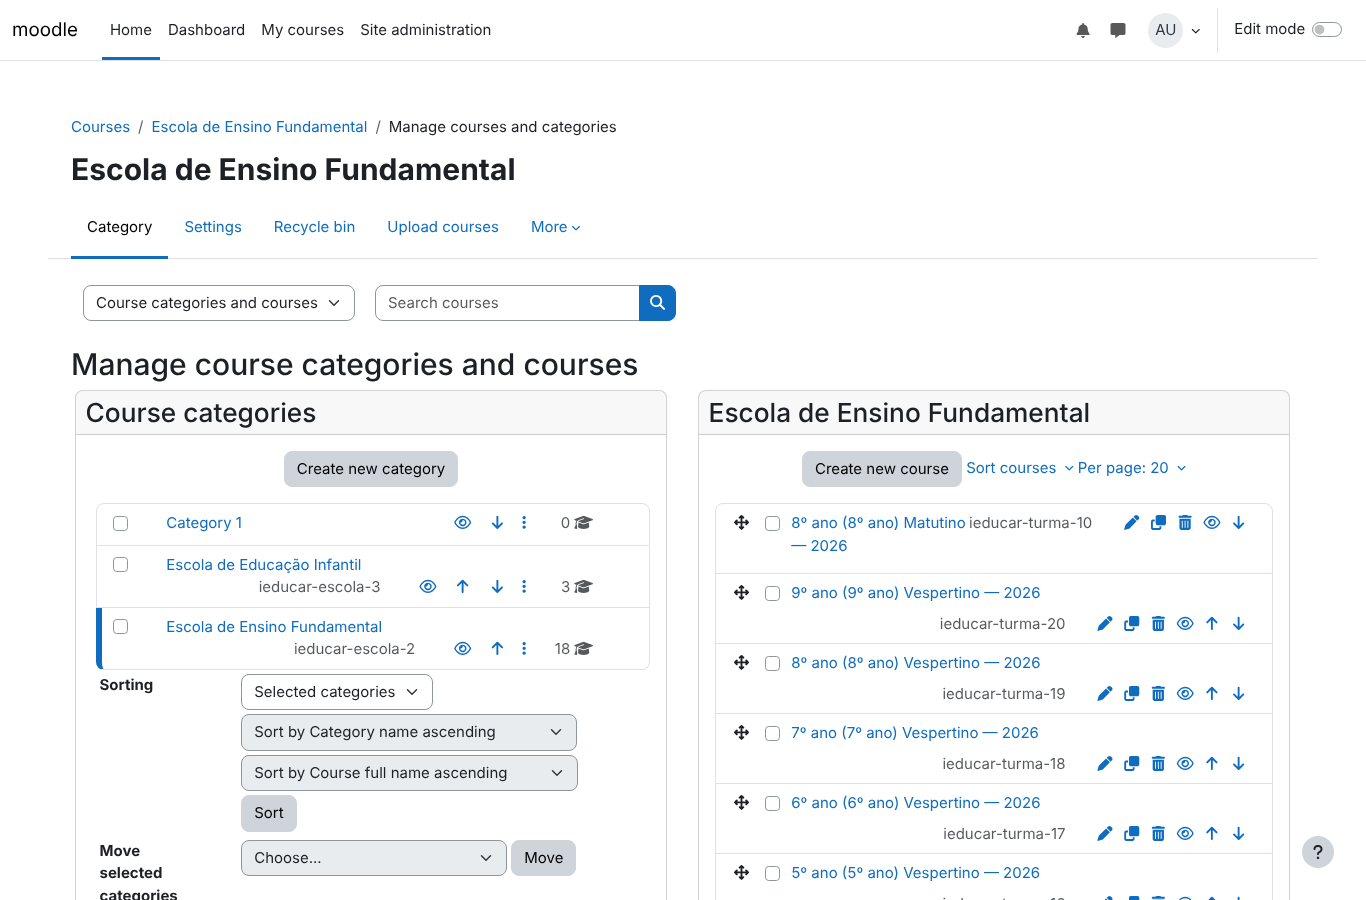
\includegraphics[width=0.92\linewidth]{figuras/moodle_cursos.png}
\caption{Resultado: categoria da escola e cursos criados no Moodle, com o \cod{idnumber} de origem}
\label{fig:moodlecursos}
\end{figure}

\begin{figure}[H]
\centering
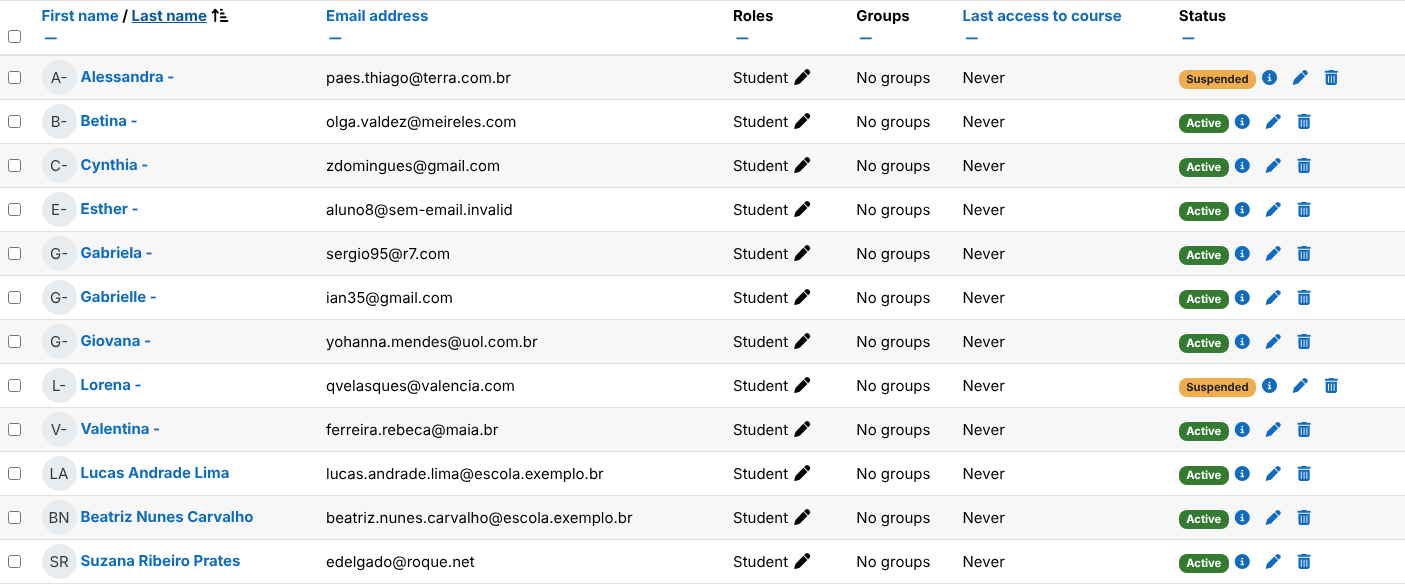
\includegraphics[width=\linewidth]{figuras/moodle_participantes.png}
\caption{Participantes de uma turma no Moodle após as alterações: alunos novos, nome corrigido, e-mail técnico para o irmão com e-mail repetido e inscrições suspensas por transferência e remanejamento}
\label{fig:participantes}
\end{figure}

\begin{figure}[H]
\centering
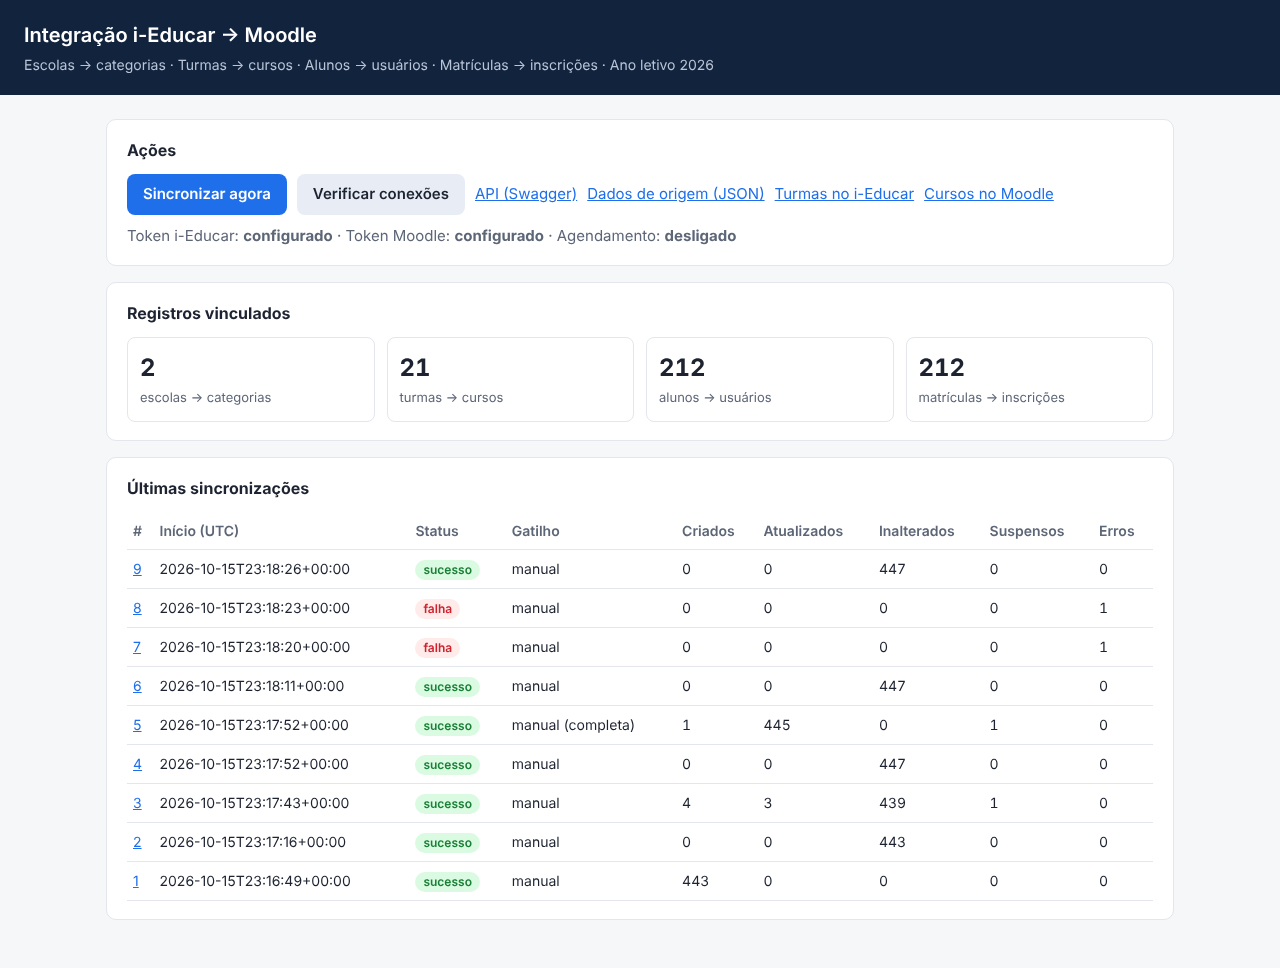
\includegraphics[width=0.85\linewidth]{figuras/painel.png}
\caption{Painel da aplicação com o histórico das execuções do roteiro}
\label{fig:painel}
\end{figure}

% ============================================================================
\section{Limitações}

\begin{itemize}
  \item \textbf{Sentido único.} Alterações feitas no Moodle em registros
    sincronizados são sobrescritas quando o dado muda na origem ou na
    reconciliação completa; nada volta ao i-Educar.
  \item \textbf{Escopo.} Professores, componentes curriculares, notas e
    frequência não são sincronizados.
  \item \textbf{Leitura completa a cada execução.} A API do i-Educar não
    oferece filtro por data de alteração; toda execução lê as matrículas do
    ano. O \emph{hash} evita escritas desnecessárias, mas o custo de leitura
    cresce com o tamanho da rede.
  \item \textbf{Detecção de mudanças no Moodle.} Exclusões feitas diretamente no
    Moodle só são corrigidas na reconciliação completa (até 1 hora).
  \item \textbf{Senhas.} Os usuários são criados com senha gerada e enviada
    pelo Moodle por e-mail; alunos com e-mail técnico não a recebem e
    precisam de outro meio de acesso (por exemplo, autenticação
    institucional).
  \item \textbf{Dependência da API do i-Educar.} A consulta de matrículas
    depende do comportamento atual do endpoint (colunas qualificadas por causa
    do \emph{JOIN}); por isso a versão do i-Educar é fixada e as respostas
    reais estão nos testes, que acusarão mudanças de formato.
  \item \textbf{Escala.} O SQLite e a trava em memória pressupõem uma única
    instância da aplicação.
  \item \textbf{Imagem do Moodle.} A \cod{bitnamilegacy/moodle} não recebe mais
    atualizações; para produção seria necessária outra imagem.
\end{itemize}

% ============================================================================
\section{Conclusão}

A integração planejada na Entrega 1 foi implementada como uma aplicação
monolítica com camadas e interfaces bem definidas, executada em um ambiente
Docker Compose completo. Ela elimina o recadastro de turmas, alunos e
matrículas no Moodle, mantém os dados consistentes ao longo do ano sem gerar
duplicidades e se recupera sozinha de falhas dos sistemas envolvidos, sem
exigir qualquer alteração no i-Educar ou no Moodle.

\bibliographystyle{sbc}
\bibliography{referencias}

\end{document}
